\begin{figure}[h]
  \centering
  \definecolor{BuiltInPKColor}{HTML}{1F77B4}
  \definecolor{BuiltInNoPKColor}{HTML}{2CA02C}
  \definecolor{SQLPKColor}{HTML}{D62728}
  \definecolor{SQLNoPKColor}{HTML}{9467BD}
  \pgfplotsset{
    tablefiveplot/.style={
      width=0.88\linewidth,
      height=0.45\linewidth,
      symbolic x coords={C1,C2,C3,C4},
      xtick=data,
      xminorticks=false,
      tick label style={font=\small},
      label style={font=\small},
    }
  }
  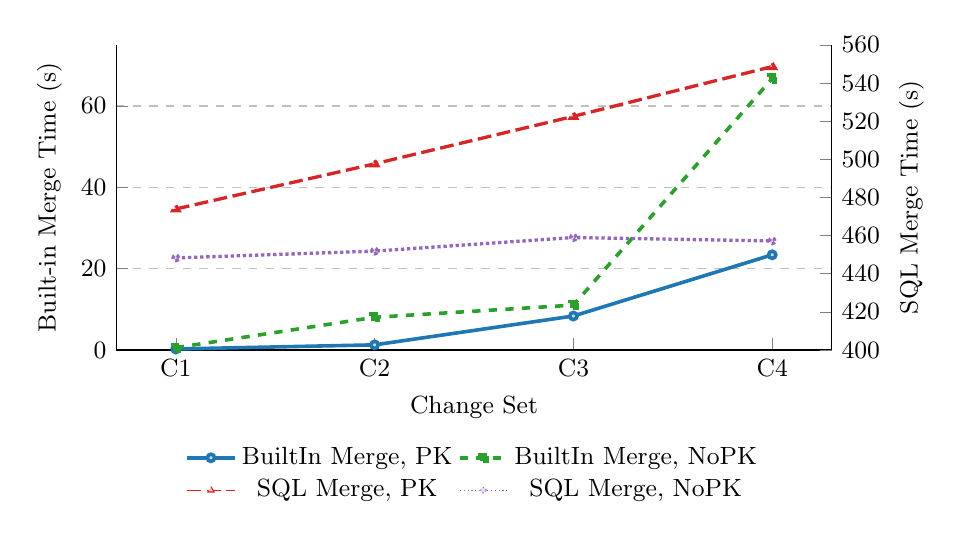
\begin{tikzpicture}
    \begin{axis}[
      tablefiveplot,
      axis y line*=left,
      axis x line*=bottom,
      ymin=0,
      ymax=75,
      xlabel={Change Set},
      ylabel={Built-in Merge Time (s)},
      ymajorgrids,
      grid style={gray!50,dashed},
      legend columns=2,
      legend style={
        font=\small,
        draw=none,
        fill=none,
        at={(0.5,-0.28)},
        anchor=north,
      },
    ]
      \addplot+[
        color=BuiltInPKColor,
        mark=*,
        mark options={scale=0.65, fill=BuiltInPKColor!25},
        line width=1.3pt,
      ]
        coordinates {(C1,0.25) (C2,1.27) (C3,8.36) (C4,23.41)};
      \addlegendentry{BuiltIn Merge, PK}
      \addplot+[
        color=BuiltInNoPKColor,
        mark=square*,
        mark options={scale=0.6},
        dashed,
        line width=1.3pt,
      ]
        coordinates {(C1,0.58) (C2,8.05) (C3,11.04) (C4,66.74)};
      \addlegendentry{BuiltIn Merge, NoPK}
      \addlegendimage{line legend, color=SQLPKColor, mark=triangle*, mark options={scale=0.65, fill=SQLPKColor!25}, dash pattern=on 5pt off 2pt}
      \addlegendentry{SQL Merge, PK}
      \addlegendimage{line legend, color=SQLNoPKColor, mark=*, mark options={scale=0.5, fill=SQLNoPKColor!25}, densely dotted}
      \addlegendentry{SQL Merge, NoPK}
    \end{axis}
    \begin{axis}[
      tablefiveplot,
      axis y line*=right,
      axis x line=none,
      ymin=400,
      ymax=560,
      ytick distance=20,
      ylabel={SQL Merge Time (s)},
    ]
      \addplot+[
        color=SQLPKColor,
        mark=triangle*,
        mark options={scale=0.65, fill=SQLPKColor!25},
        dash pattern=on 5pt off 2pt,
        line width=1.2pt,
      ]
        coordinates {(C1,473.96) (C2,497.65) (C3,522.54) (C4,548.66)};
      \addplot+[
        color=SQLNoPKColor,
        mark=*,
        mark options={scale=0.5, fill=SQLNoPKColor!25},
        densely dotted,
        line width=1.2pt,
      ]
        coordinates {(C1,448.30) (C2,451.87) (C3,459.00) (C4,457.21)};
    \end{axis}
  \end{tikzpicture}
  \caption{Line chart summarizing Table~\ref{tab:expmerge42} results.}
  \label{fig:table7-line}
\end{figure}
